\chapter{Referencial Teórico}

A principal ferramenta para modelar o nosso problema surgiu em 1736. Nessa época existia a cidade de Königsberg (atual Kaliningrado), representada pela Figura \ref{Konigsberg}, por ela passava o Rio Prególia que separava a cidade em 4 partes. Para se caminhar livremente pelas 4 regiões foram construídas 7 pontes que ligavam cada região. Isso gerava uma dúvida entre os moradores: seria possível sair de uma região e voltar para ela passando por todas as pontes apenas uma vez?

Leonhard Euler~\cite{Euler1736} se interessou pelo assunto e tentou resolver esse problema. Para isso ele criou uma estrutura chamada Grafo que era composto por pontos (nós) que representavam as regiões e 
ligações entre esses pontos  
que representavam as pontes entre as regiões 
e ignorou toda a forma geométrica de cada um desses objetos. Euler percebeu que para que haja esse caminho é necessário e suficiente que todos os nós tenham um número de ligações pares. Pois para haver uma solução deve existir um caminho de ida e um de volta para cada vértice, como isso não é verdade para a cidade de Königsberg, então 
não é possível sair de uma região e voltar para ela passando uma única vez em cada ponte de Königsberg.

\begin{figure}[H]
  \centering
  \captionsetup{font=normalsize,skip=1pt,singlelinecheck=on,labelsep=endash}
  \caption{Pontes de Königsberg}
  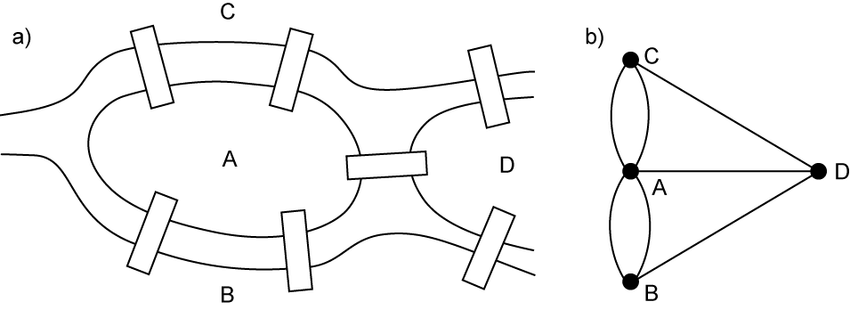
\includegraphics[scale=0.5]{figuras/Koenigsberg.png}
  \captionsetup{font=small,position=below,skip=-1pt}
   \caption*{Fonte: Boguslawski, Pawel~\cite{Koenigsberg}.}
   \label{Konigsberg}
\end{figure}

A prova de Euler mostra que quando se quer modelar algum problema não é necessário considerar todas as variáveis existentes neles, mas o essencial para a solução. Nesse caso o mais importante foi esquematizar o problema usando Grafos e, principalmente, analisar uma estrutura intrínseca ao Grafo.

Com a solução do problema surge a área da matemática chamada Grafos que é a base matemática para o que chamamos em redes. Essa nomenclatura varia de área para área; na física, por exemplo, são sinônimos enquanto na computação Grafos estão relacionados à problemas de fluxo~\cite{Grafos01,Grafos} e redes são utilizados para problemas visando a estrutura do Grafo e suas interações~\cite{network,networks}. Nesse trabalho usaremos os dois como sinônimos.

\section{Conceitos Fundamentais}

Um Grafo $G(\mathpzc{N} ,\mathpzc{L})$ é uma dupla na qual $\mathpzc{N} = \{\nu_0,\nu_1,\nu_2,...,\nu_i,...\}$ é um conjunto não vazio de elementos chamados de vértices ou 
nós e $\mathpzc{L}$ é um conjunto não vazio de pares 
de elementos de $\mathpzc{N}$ chamados de 
arestas ou ligações. Dessa forma podemos definir $N = |\mathpzc{N}|$ que mensura a quantidade de vértices que há em $G$ e $L= |\mathpzc{L}|$ que mensura o número de arestas. Essas quantidades também são chamadas de ordem e tamanho~\cite{Grafos}, respectivamente.

A partir dessa definição de redes é possível definir a Matriz de Adjacência que guarda a informação de 
conexões entre os nós. Seja uma matriz $A$ quadrada de tamanho $N \times N$, cada elemento da matriz segue a seguinte regra:
\[   
  A_{i,j} = 
     \begin{cases}
       1 \quad 
       \text{se } (\nu_i,\nu_j)\in \mathpzc{L}\\
       0 \quad \text{caso contrário.} \\
     \end{cases}
\]

A partir dela surgem características importantes de redes. Se $A_{i,j} = A_{i,j}\; \forall \nu_i,\nu_j \in \mathpzc{N}$ então a rede é chamada de não direcionada; se $\exists \nu_i\neq \nu_j$ tal que 
$A_{i,j} \neq A_{j,i}$ 
ela é chamada de direcionada. Isso pode ter diferentes interpretações a depender do contexto, por exemplo na rede de amigos do \textit{Facebook}, se o usuário A é amigo de B, então B é amigo de A. No caso do \textit{Instagram} se A segue B, não necessariamente B segue A. No primeiro caso é natural modelarmos utilizando redes não direcionadas, enquanto no segundo usamos redes direcionadas.

Uma alternativa para registrar a informação da Matriz de Adjacência é através da lista de vizinhos. Dois vértices $\nu$ e $\mu$ são vizinhos se existe uma ligação entre $\nu$ e $\mu$, assim é denotado $\eta(\nu)$ o conjunto de vizinhos do vértice $\nu$ para redes não direcionadas. Em redes direcionadas, existem dois tipos de vizinhos: os que se conectam a um nó e os que são conectados por um nó. Portanto, denotaremos $\eta_{in}(\nu)$ todos os vizinhos que têm ligação que chega em $\nu$ e $\eta_{out}(\nu)$ todos os vizinhos que têm ligação que sai de $\nu$.

Por fim, é possível adicionar propriedades às nossas ligações. As propriedades têm várias interpretações nos problemas: em uma rede de canos de esgoto, o fluxo que passa em um cano pode ser um peso e em redes de \textit{Facebook} o nível de amizade pode ser um peso das ligações entre usuários. 
Além disso, pode-se também adicionar pesos aos vértices, representando alguma característica não-topológica dos mesmos, como, exemplo, idade de um indivíduo.
Formalmente, um Grafo ponderado $G(\mathpzc{N},\mathpzc{L},\Theta,\Xi\left(\nu_i,\nu_j\right))$ é formado por um conjunto de nós $\mathpzc{N}$, um conjunto de arestas $\mathpzc{L}$ e um mapeamento $\Theta: \mathpzc{N}\mapsto \mathpzc{S}$ que representa uma rede ponderada nos nós e 
$,\Xi\left( \nu,\mu \right): \mathpzc{L}\mapsto \mathpzc{R}$ na qual $\mathpzc{R}$ e $\mathpzc{S}$ são propriedades da rede que podem ser quantitativas ou qualitativas, vetoriais ou não. Nesse caso é definido uma generalização da matriz da Matriz de Adjacência, seja 
$w_{\nu,\mu}$ o peso da ligação $(\nu,\mu$) então definimos a Matriz de Adjacência Ponderada como:
\[   
  W_{i,j} = 
     \begin{cases}
       w_{\nu_i,\nu_j} \quad 
       \text{se } (\nu_i,\nu_j)\in \mathpzc{L}\\
       0 \quad \text{caso contrário.} \\
     \end{cases}.
\]

A Figura \ref{fig:redes} mostra um exemplo 
de uma rede com 8 nós enumerados de 0 a 7, com 12 arestas e a matriz de adjacência $A_{i,j}$ .

\begin{figure}[H]
  \centering
  \captionsetup{font=normalsize,skip=0.8pt,singlelinecheck=on,labelsep=endash}
  \caption{Ilustração de Redes e seus Parâmetros}
  \begin{tikzpicture}[make origin horizontal center of bounding box]
    \draw[black, thick] (0,0) -- ($(2,0)+(0,1.5)$);
    \draw[black, thick] (0,0) -- ($(-2,0)+(0,2)$);
    \draw[black, thick] (0,0) -- ($(-2,0)+(0,-1)$);
    \draw[black, thick] (0,0) -- ($(-3.5,0)+(0,-1)$);
    \draw[black, thick] (-3.5,-1) -- ($(-4,0)+(0,1)$);
    \draw[black, thick] (-2,-1) -- ($(-4,0)+(0,1)$);
    \draw[black, thick] (-4,1) -- ($(-2,0)+(0,2)$);
    \draw[black, thick] (-2,-1) -- (-3.5,-1);
    \draw[black, thick] (-4,1) -- (-5.5,0);
    \draw[black, thick] (-3.5,-1) -- (-5.5,0);
    \draw[black, thick] (-4,1) -- (-5.5,-2.5);
    \draw[black, thick] (-3.5,-1) -- (-5.5,-2.5);

    \draw[black, fill=white] ($(0,0) + (0,0)$) circle [radius=0.3] node {0};
    \draw[black, fill=white] ($(2,0) + (0,1.5)$) circle [radius=0.3] node {1};
    \draw[black, fill=white] ($(-2,0) + (0,2)$) circle [radius=0.3] node {5};
    \draw[black, fill=white] ($(-2,0) + (0,-1)$) circle [radius=0.3] node {2};
    \draw[black, fill=white] ($(-4,0) + (0,1)$) circle [radius=0.3] node {4};
    \draw[black, fill=white] ($(-5.5,0) + (0,0)$) circle [radius=0.3] node {6};
    \draw[black, fill=white] ($(-3.5,0) + (0,-1)$) circle [radius=0.3] node {3};
    \draw[black, fill=white] ($(-5.5,0) + (0,-2.5)$) circle [radius=0.3] node {7};
    
    \node at (4,3) {$N = 8$};
    \node at (4,2.5) {$L = 12$};
    \node at (2.5,-1) {$A = $};
    \draw [decorate,
    decoration = {brace}] (3,-3.2) --  (3,1.2);
    \draw [decorate,
    decoration = {brace, mirror}] (7,-3.2) --  (7,1.2);
    \matrix at (5,-1)
  {

    \node {0}; & \node{1}; & \node {1}; & \node {1}; & \node {0}; & \node {1}; & \node {0}; & \node {0};  \\
    
    \node {1}; & \node{0}; & \node {0}; & \node {0}; & \node {0}; & \node {0}; & \node {0}; & \node {0};  \\

    \node {1}; & \node{0}; & \node {0}; & \node {1}; & \node {1}; & \node {0}; & \node {0}; & \node {0};  \\

    \node {1}; & \node{0}; & \node {1}; & \node {0}; & \node {1}; & \node {0}; & \node {1}; & \node {1};  \\

    \node {0}; & \node{0}; & \node {1}; & \node {1}; & \node {0}; & \node {1}; & \node {1}; & \node {1};  \\

    \node {1}; & \node{0}; & \node {0}; & \node {0}; & \node {1}; & \node {0}; & \node {0}; & \node {0};  \\

    \node {0}; & \node{0}; & \node {0}; & \node {1}; & \node {1}; & \node {0}; & \node {0}; & \node {0};  \\
    
    \node {0}; & \node{0}; & \node {0}; & \node {1}; & \node {1}; & \node {0}; & \node {0}; & \node {0};  \\
  };
  \end{tikzpicture}
  \captionsetup{font=small}
  \caption*{Ilustração de uma rede, das suas quantidades de ligações $L$, de nós $N$ e da Matriz de Adjacência $A$.\\ Fonte: Elaborado pelo autor}
  \label{fig:redes}
\end{figure}

\section{Métricas estruturais de Redes}

Como discutido anteriormente é muito importante estudarmos a estrutura da rede.
Para um entendimento melhor dessa estrutura existem várias métricas~\cite{Costa2007} relacionadas à topologia da rede podendo ser classificadas como globais ou locais. 
Métricas globais de redes são medidas que fornecem informações sobre as propriedades e características de uma rede como um todo, em oposição às métricas locais que se concentram em elementos individuais dentro da rede, como nós ou arestas. 
Ao final
desta seção, a Figura \ref{Exemplo01} e as Tabelas \ref{tab:Global}-\ref{tab:centralidade_rede} apresentam um exemplo com aplicações dessas métricas.

\subsection{Métricas Globais de Redes}

Seja \( G' \) um grafo \( G'(\mathpzc{N}', \mathpzc{L}') \) tal que \( \mathpzc{N}' \subseteq \mathpzc{N} \) e \( \mathpzc{L}' \subseteq \mathpzc{L} \), \( G' \) então é definido como sub-grafo de $G$, pois contém vértices e arestas que também estão em $G$ . Assim uma componente de um grafo \( G \) como um subgrafo que satisfaz duas condições: conectividade interna e maximalidade. Conectividade interna significa que, para qualquer par de vértices \( u, v \in C \), existe um caminho em \( C \) que conecta \( u \) a \( v \) usando apenas vértices e arestas de \( C \), ou seja, o subgrafo induzido por \( C \) é conexo. Maximalidade implica que não é possível adicionar nenhum outro vértice ou aresta ao subgrafo \( C \) sem perder a propriedade de conectividade interna, ou seja, \( C \) é maximal com respeito à conectividade.


Sejam dois vértices $\nu,\mu \in \mathpzc{N}$ é dito que existe um caminho entre $\nu$ e $\mu$ se existe uma sequência de vértices $\zeta_1,\zeta_{2},...,\zeta_m | (\zeta_{s},\zeta_{s+1}) \in \mathpzc{L}$, $\zeta_1=\nu$, $\zeta_m=\mu$, na qual não há repetição de vértices ou arestas. O comprimento de um caminho é dado por sua quantidade de arestas. 
Podem existir vários caminhos 
entre $\nu$ e $\mu$, portanto a distância geodésica entre dois vértices $d_{\nu,\mu}$ é definida como o menor comprimento dentre todos os caminhos entre $\nu$ e $\mu$. Mediante essa definição, é possível construir a métrica 
global $\left\langle d \right\rangle $
chamada distância geodésica média da rede:
\begin{equation}
     \left\langle d \right\rangle  = \sum_{\substack{\nu\neq\mu}} \frac{d_{\nu,\mu}}{N\cdot(N-1)}.
\end{equation}
Esse valor nos dá a informação sobre o quanto em média é necessário caminhar na rede de um nó para outro. No caso de redes ponderadas considere dois vértices $\nu,\mu \in \mathpzc{N}$ é dito que existe um caminho entre os dois nós se existe uma sequência de vértices $\zeta_1,\zeta_{2},...,\zeta_m | (\zeta_{s},\zeta_{s+1}) \in \mathpzc{L}$, $\zeta_1=\nu$, $\zeta_m=\mu$ e para esse caminho é atribuído um peso $\sum_{s}w_{\zeta_s,\zeta_{s+1}}$, portanto o menor caminho é aquele que minimiza 
$\sum_{s}w_{\zeta_s,\zeta_{s+1}}$ e seu valor será a distância geodésica $d_{\nu,\mu}^w$. Contudo a concepção de menor caminho entre dois pontos pode depender do problema, por exemplo para se achar a resistência equivalente em uma rede de resistores pode se utilizar da mínima resistência ou de máxima corrente.

Outro valor importante é o chamado diâmetro $d = \max\limits_{\nu,\mu} d_{\nu,\mu}$ que é a maior distância geodésica da rede, ele reflete o maior número de etapas necessárias para viajar entre os dois vértices mais distantes na rede, fornecendo uma medida da ``extensão'' da rede em termos da sua conectividade. 
Esse valor está relacionado a um tipo de rede chamada redes de pequeno mundo, \citeonline{Watts1998} definem que uma rede é dita de pequeno mundo quando $\left\langle d\right\rangle \propto \log(N)$, redes com essa propriedades apresentam uma pequena distância entre qualquer par de nós e facilmente a informação pode propagar na rede.

Uma outra métrica a ser avaliada é o número de conexões que cada nó contém. É definido o grau $k_{\nu}$ como o número de conexões (ou vizinhos) que o nó $\nu$ possui para redes não direcionadas. Para redes direcionadas existe uma divisão entre $k^{in}_{\nu}$ e $k^{out}_{\nu}$ para os nós que pertencem a $\eta_{in}(\nu)$ e $\eta_{out}(\nu)$, respectivamente. Pode-se achar os valores $k^{in}_{\nu_i}$ e $k^{out}_{\nu_i}$ a partir da Matriz de Adjacência da seguinte forma:
\begin{equation}
    k^{in}_{\nu_i} = \sum_{j} A_{j,i}, \qquad  k^{out}_{\nu_i} = \sum_{j} A_{i,j}.
\end{equation}
Nessa formulação é possível definir o grau em redes ponderadas  
$k^w_{\nu_i}$ substituindo $A_{i,j}$ por $W_{i,j}$. 
Além disso é possível também definir o grau médio $\left\langle k \right\rangle$ da rede
\begin{equation}
  \left\langle k \right\rangle = \sum\limits_{\nu\in\mathpzc{N}}\frac{k_{\nu}}{N} = 2\frac{L}{N}.
  \label{grau_tamanho}
\end{equation}
Esse valor tem bastante importância quantitativa quando o objetivo é trabalhar com distribuições de graus.
Analogamente, pode-se definir o grau de entrada ou de saída médio, bem como o grau ponderado médio da rede.

Outras duas métricas importantes são a densidade $\rho(G)$ e a reciprocidade $rc(G)$. A primeira mede a razão entre a quantidade de arestas dentro do grafo $G$ pela quantidade total de arestas que o grafo pode suportar. Já a segunda nos apresenta a fração de arestas que existem em ambas as direções; no caso trivial de redes não direcionadas esse valor é igual a 1.
\[   
  \rho(G) = 
     \begin{cases}
      \frac{2L}{N\cdot(N-1)} \quad \text{se a rede for não direcionada, ou }\\
      \frac{L}{N\cdot(N-1)} \quad \text{se a rede for direcionada;} \\
     \end{cases}
\]
\begin{equation}
  rc(G) = \frac{\sum\limits_{i,j} A_{i,j}A_{j,i}}{\sum\limits_{i,j } A_{i,j}}.
\end{equation}

Por fim existe uma métrica para analisar o Agrupamento de uma Rede, ou seja quanto que os vértices estão unidos. Essa métrica será definida a partir da probabilidade de um vizinho do nó $\nu_i$ estar conectado com outro vizinho de $\nu_i$
\begin{equation}
  C(G) = \frac{\sum\limits_{(i,j,k): i\neq j \neq k}A_{i,j}A_{j,k}A_{k,j}}{\sum\limits_{(i,j,k): i\neq j \neq k}A_{i,j}A_{j,k}} = 3\frac{\#\text{Triângulos}}{\#\text{Tríades}},
  \label{clustering2}
\end{equation}
em que $\#$ significa número de alguma coisa, no caso estamos contando o número de triângulos e o número de tríades que aparecem na rede. Essa é a definição do que chamamos de Agrupamento Global, podemos também definir o Agrupamento Local $C(\nu)$ e por ele o Agrupamento Médio $\langle C\rangle$:
\begin{equation}
  C(\nu) = 2\frac{\#\text{Triângulos que contém o nó }\nu}{\#\text{Tríades que contém o nó }\nu}, \qquad   \langle C \rangle = \sum\limits_{\nu \in \mathpzc{N}}\frac{C(\nu)}{N}.
  \label{clusteringlocal}
\end{equation}

A Figura~\ref{Exemplo01} ilustra uma rede e 
  suas Métricas Globais: menor caminho médio $\langle d \rangle$, diâmetro $d$, grau médio $\langle k \rangle$, densidade $\rho$, Agrupamento $C$, Agrupamento Médio $\langle C \rangle$. Os valores do \#Triângulos, \#Triades e o Agrupamento se encontram na Tabela \ref{tab:Global}.

\begin{figure}[H]
  \centering
  \captionsetup{font=normalsize,skip=0.8pt,singlelinecheck=on,labelsep=endash}
  \caption{Ilustração de Redes e suas Métricas Globais. Fonte: Elaborado pelo autor}
  \begin{tikzpicture}[make origin horizontal center of bounding box]
    \draw[black, thick] (0,0) -- ($(2,0)+(0,1.5)$);
    \draw[black, thick] (0,0) -- ($(-2,0)+(0,2)$);
    \draw[black, thick] (0,0) -- ($(-2,0)+(0,-1)$);
    \draw[black, thick] (0,0) -- ($(-3.5,0)+(0,-1)$);
    \draw[black, thick] (-3.5,-1) -- ($(-4,0)+(0,1)$);
    \draw[black, thick] (-2,-1) -- ($(-4,0)+(0,1)$);
    \draw[black, thick] (-4,1) -- ($(-2,0)+(0,2)$);
    \draw[black, thick] (-2,-1) -- (-3.5,-1);
    \draw[black, thick] (-4,1) -- (-5.5,0);
    \draw[black, thick] (-3.5,-1) -- (-5.5,0);
    \draw[black, thick] (-4,1) -- (-5.5,-2.5);
    \draw[black, thick] (-3.5,-1) -- (-5.5,-2.5);

    \draw[black, fill=white] ($(0,0) + (0,0)$) circle [radius=0.3] node {0};
    \draw[black, fill=white] ($(2,0) + (0,1.5)$) circle [radius=0.3] node {1};
    \draw[black, fill=white] ($(-2,0) + (0,2)$) circle [radius=0.3] node {5};
    \draw[black, fill=white] ($(-2,0) + (0,-1)$) circle [radius=0.3] node {2};
    \draw[black, fill=white] ($(-4,0) + (0,1)$) circle [radius=0.3] node {4};
    \draw[black, fill=white] ($(-5.5,0) + (0,0)$) circle [radius=0.3] node {6};
    \draw[black, fill=white] ($(-3.5,0) + (0,-1)$) circle [radius=0.3] node {3};
    \draw[black, fill=white] ($(-5.5,0) + (0,-2.5)$) circle [radius=0.3] node {7};
    
    \node at (4,1.25) {$\langle l \rangle = 
    1.68$};
    \node at (4,0.75) {$d = 3$};
    \node at (4,0.25) {$\langle k \rangle = 
    3$};
    \node at (4,-0.25) 
{$\rho = 12/28$};
    \node at (4,-0.75) {$C = 0.375$};
    \node at (4,-1.25) {$ \langle C \rangle 
    = 0.4417$};
  \end{tikzpicture}
  \label{Exemplo01}
\end{figure}

\begin{table}[H]
    \captionsetup{font=normalsize,skip=0.8pt,singlelinecheck=on,labelsep=endash}
\caption{Valores de \#Triângulos($\nu_i$), \#Tríades($\nu_i$)  e $C(\nu_i)$ do exemplo da Figura \ref{Exemplo01}.}

    \centering
    \begin{tabular}{|c|c|c|c|c|c|c|c|c|}%
        \hline%
         nó &0&1&2&3&4&5&6&7\\%         
        \hline%
    \#Triângulos($\nu_i$)&1&0&2&4&3&0&1&1\\%
        \hline%
        \#Tríades($\nu_i$)&6&0&3&10&10&1&1&1\\%%\#Triades(\nu_i)&6&0&3&10&0&10&1&1\\%
        \hline%
        \#C($\nu_i$)&0.167&0.000&0.667&0.400&0.300&0.000&1.000&1.000\\%
        \hline%
    \end{tabular}%
    \label{tab:Global}
\end{table}



\subsection{Métricas Locais de Centralidade}


Ao estudar redes o interesse está voltado em entender suas estruturas e propriedades, isso já é possível dadas as métricas que apresentamos anteriormente. É importante destacar que essas métricas globais oferecem uma análise abrangente da topologia da rede, revelando suas propriedades e comportamentos coletivos que podem estar diluídas na rede ou concentradas em nós específicos. Portanto estudar os nós em si e a sua importância perante a rede é necessário; para isso são usadas as chamadas Métricas Locais de Centralidade. 

Quando falamos de Métricas de Centralidade o interesse é estudar a importância topológica de cada nó perante a rede. 
Mas em que sentido seria essa importância? Depende do problema, talvez seja necessário estudar qual o autor mais importante em uma rede de citações de artigos~\cite{Leydesdorff2011} ou qual indivíduo devemos retirar de uma rede criminosa para desfazer a rede~\cite{deAndrade2021}. Para ambos os casos e vários outros exemplos existem métricas apropriadas para atingir tais objetivos.

A métrica inicial a ser analisada consiste na contagem das conexões individuais de cada nó, representada pelo grau $k_\nu$. Ao conduzir essa avaliação, identificamos o nó central como aquele que apresenta o grau $k_\nu$ mais elevado, objetivando, assim, encontrar o nó com a maior quantidade de conexões que é a Centralidade de Grau (CG).

A segunda métrica importante é a Centralidade de Excentricidade (CE). Essencialmente, a CE de um nó é determinada calculando-se o recíproco da maior distância que separa esse nó de qualquer outro nó na rede. Ela exibe a distância máxima que um nó precisa percorrer para alcançar o ponto mais remoto da rede. O nó cuja maior distância é a menor entre todos os nós da rede é então identificado como o mais central. Formalmente $CE(\nu)\; \forall \nu \in \mathpzc{N}$ é definida como:
\begin{equation}
  CE(\nu) = \frac{1}{\max\limits_{\mu} d_{\nu,\mu}}.
\end{equation}
Nessa mesma ideia é propício avaliar outras duas métricas parecidas: Centralidade de Proximidade (CP) e Centralidade Harmônica (CH). Em ambas o interesse é entender qual é o nó mais central a partir de quanto ele dista dos outros, a diferença entre as duas é que a primeira é calculada pelo inverso da média aritmética e a segunda com a média harmônica:
\begin{equation}
  CP(\nu) = \frac{N - 1}{\sum\limits_{\mu \neq \nu} d_{\nu,\mu}},
\end{equation}
\begin{equation}
  CH(\nu) = \frac{1}{N - 1}\sum_{\mu \neq \nu}\frac{1}{d_{\nu,\mu}}.
\end{equation}

Uma generalização da CP e CE é a Centralidade de
Média-$p$ ($C_p$)~\cite{Andrade2019}. A ideia desta medida de centralidade é usar a noção de média
generalizada das distâncias. Ela é definida como:
\begin{equation}
  C_p(\nu) = 
  \begin{cases}
    \left(\frac{\sum\limits_{\mu \neq \nu } d_{\nu,\mu}^p}{N - 1}\right)^{-\frac{1}{p}} &\text{se $p \neq 0$},\\
    \left(\prod\limits_{\mu \neq \nu} d_{\nu,\mu}\right)^{-\frac{1}{N - 1}} &\text{se }p = 0.
  \end{cases}
\end{equation}

Entretanto a importância de um nó não está associada somente a sua distância 

com os outros nós da rede, existem aqueles que são importantes por 

intermediarem
conexões entre nós. Por exemplo,
considere a rede mundial
de 
aeroportos, que seja construída a partir de nós como sendo os aeroportos e as ligações sendo as viagens entre aeroportos. Nessa situação, imagine que tenha um país altamente conectado entre si, contudo ele só tem um aeroporto que liga esse país ao exterior, esse nó é importante não pela distância dele para os outros aeroportos mas porque ele é o principal e 
a única conexão
entre o exterior e o país.

Para ser possível detectar e mensurar esse tipo de importância, considere
$\mathbb{L}_{\mu,\zeta}$ o número de caminhos mínimos que vão de $\nu$ para $\mu$ e 
$\mathbb{L}^{\nu}_{\mu,\zeta}$ 
o número de mínimos caminhos entre $\mu$ e $\zeta$ e passam pelo vértice
$\nu$. Portanto, podemos definir a Centralidade de Intermediação ($CB$) como
\begin{equation}
  CB(\nu) = \frac{1}{(N - 1)(N - 2)} \sum\limits_{\mu \neq \zeta} \frac{\mathbb{L}^{\nu}_{\mu,\zeta}}{\mathbb{L}_{\mu,\zeta}},
\end{equation}
em que $\mu$ e $\zeta$ são diferentes do nó $\nu$.

Quando se trata de analisar uma rede empresarial, é fundamental reconhecer a relevância do CEO para a organização. No entanto, é importante notar que o CEO mantém comunicação direta apenas com os líderes de cada região da empresa, enquanto esses líderes não necessariamente se comunicam diretamente entre si. Portanto, onde reside a indicação da importância do CEO? A resposta a essa indagação repousa no fato de que o CEO estabelece conexões com indivíduos influentes na rede, um aspecto que não é capturado pelas métricas 
mencionadas até então
de análise de rede. Definimos a Centralidade de Autovetor ($CA$) como:
\begin{equation},
  CA(\nu_i) = \frac{1}{\lambda}\sum_{\nu_j}A_{i,j}\; CA(\nu_j),
\end{equation}
na qual $\lambda$ é o maior autovalor associado à matriz de adjacência de rede. A importância dessa conexão é que os autovetores e autovalores capturam informações sobre como a informação flui na rede. Se um nó estiver conectado a outros nós importantes (ou seja, nós com alta centralidade), ele terá uma alta centralidade de autovetor, mesmo que tenha poucas conexões diretas. Em contrapartida, se um nó estiver conectado principalmente a nós periféricos, terá uma baixa centralidade de autovetor.

Com o advento das páginas da \textit{internet} é preciso metrificar quais são os \textit{sites} mais importantes. Para isso seria importante não só levar em consideração quem está em posição privilegiada, mas também como essa posição é mitigada pelo número de ligações, portanto~\cite{page1999pagerank} publicaram uma nova métrica que consegue quantificar isso chamada de \textit{PageRank}. Essa métrica é utilizada pelo \textit{Google} para analisar a importância de \textit{sites} na \textit{internet}. Considere um usuário que navega pela \textit{internet} e está em um \textit{site} $\nu_j$ e deseja ir para outro. Existe uma probabilidade $\alpha$ de o usuário seguir um \textit{link} dentro do \textit{site} atual e ir para outro que ele aponta, e uma probabilidade $1 - \alpha$ de ele não seguir essa estrutura e ir para um \textit{site} aleatório. Eles definiram o \textit{PageRank} do nó $\nu_j$ como:
\begin{equation}
    PR(\nu_j) =1 - \alpha + \alpha\times \sum_{j \neq i} A_{i,j}\frac{PR(\nu_i)}{k^{out}_{\nu_j}}.
\end{equation}

\citeonline{Carmi2007} formularam o algoritmo \textit{K-Shell} que se concentra em decompor a rede não direcionada em camadas, onde cada camada representa um subconjunto de nós com uma centralidade mínima, conhecida como o ``grau mínimo'' K. Inicialmente, os nós são ordenados por grau em ordem decrescente, e aqueles com menor grau são iterativamente removidos até que nenhum nó com grau menor ou igual a K permaneça na rede. Esse processo gera uma sequência de camadas (\textit{K-Shells}), onde as camadas mais internas contêm nós de alta centralidade, enquanto as camadas mais externas contêm nós de menor centralidade. 
O seguinte algoritmo realiza a descomposição em \textit{K-Shells}: 
\begin{enumerate}
    \item É inicializado \( k = 1 \). Este é o nível inicial de k-shell.
    \item Encontre e remova todos os vértices de grau \( k \). Atribua a esses vértices o k-shell \( k \).
    \item Após a remoção, reduza em 1 o grau de todos os vértices adjacentes aos removidos.
    \item Se ainda existirem vértices de grau \( k \) no grafo residual, repita o passo 2 e 3 para esses vértices.
    \item Incremente \( k \) para \( k + 1 \) e verifique se existem vértices de grau \( k \) no grafo residual. Se sim, repita os passos 2 a 4.
    \item Continue o processo até que não reste nenhum vértice no grafo.
    \item O algoritmo termina quando todos os vértices são atribuídos a um k-shell e o grafo está completamente decomposto.
\end{enumerate}

A tabela \ref{tab:centralidade_rede} apresentada resume os valores de diferentes métricas de centralidade para uma rede específica, conforme ilustrado na Figura \ref{fig:redes}. Cada coluna representa um nó individual da rede, numerados de 0 a 7, e cada linha descreve uma métrica específica de centralidade: Centralidade de Excentricidade (CE), Centralidade de Grau (CG), K-shell (CK), Centralidade de Proximidade (CP), Centralidade de Harmonia (CH), Centralidade de Betweenness (CB) e Centralidade de Autovalor (CA). Observa-se uma variabilidade entre os nós nas medidas de Centralidade de Excentricidade (CE), com nós como o 1, 5, 6 e 7 exibindo valores inferiores, indicando uma posição mais periférica na rede. O nó 3 destaca-se com valores altos tanto na Centralidade de Grau (CG) quanto na Centralidade de Betweenness (CB), sublinhando sua influência central como ponto de conexão e intermediário crucial nas interações da rede.
\begin{table}[H]
    \captionsetup{width=13.5cm}
    \caption{Valores de diferentes métricas de centralidade do exemplo da Figura \ref{Exemplo01}.}
    \centering
    \begin{tabular}{crrrrrrrr}
        \toprule
        & nó 0 & nó 1 & nó 2 & nó 3 & nó 4 & nó 5 & nó 6 & nó 7 \\
        \midrule
        \midrule
        CE & 0.5 & 0.333 & 0.5 & 0.5 & 0.5 & 0.333 & 0.333 & 0.333 \\
        CG & 0.571 & 0.143 & 0.429 & 0.714 & 0.286 & 0.714 & 0.286 & 0.286 \\
        CK & 2 & 1 & 2 & 2 & 2 & 2 & 2 & 2 \\
        CP & 0.7 & 0.438 & 0.636 & 0.778 & 0.583 & 0.7 & 0.538 & 0.538 \\
        CH & 5.5 & 3.5 & 5.0 & 6.0 & 5.833 & 4.5 & 4.333 & 4.333 \\
        CB & 0.333 & 0.0 & 0.032 & 0.294 & 0.032 & 0.214 & 0.0 & 0.0 \\
        CA & 0.353 & 0.101 & 0.385 & 0.511 & 0.239 & 0.486 & 0.285 & 0.285 \\
        \bottomrule
    \end{tabular}
    \caption*{Valores de diferentes métricas de centralidade calculados para a rede ilustrada na Figura \ref{fig:redes}, os valores foram calculados utilizando a biblioteca Networkx.\\ Fonte:~\cite{hagberg2008exploring}.}
    \label{tab:centralidade_rede}
\end{table}

\subsection{Métricas em Redes Ponderadas}

Na seção anterior, foram discutidas diversas métricas tradicionais empregadas na análise de redes e grafos. Embora essas métricas sejam fundamentais e amplamente reconhecidas no campo da análise de redes, é importante reconhecer que elas apresentam limitações. As suas principais dificuldades estão em ao considerar ponderação nas arestas metrificar somente com viés de estrutura da rede e pouco se leva em conta uma real mistura entre esses dois valores. 

\citeonline{Rgo2019} criaram uma métrica para estudar co-autoria em artigos acadêmicos levando em conta a força entre as ligações dos vizinhos de cada autor e também como essa ligação é importante perante outras ligações entre vizinhos. A 
métrica de Utilidade é definida como:
\begin{equation}
    U(\nu) = \sum_{\substack{\mu \in \eta(\nu)}} \left(\frac{w_{\nu,\mu}}{k^w_\nu}+ \frac{w_{\nu,\mu}}{k^w_\mu} + \frac{w_{\nu,\mu}^2}{k^w_\nu k^w_\mu}\right)
\end{equation}
O primeiro termo quantifica o quão importante é a ligação entre o sítio $\nu$ com $\mu$ em relação às ligações de $\nu$, já o segundo é em relação às ligações de $\mu$ e o terceiro termo é um termo misto. Para redes sem ponderação $w_{\nu,\mu} = 1$, $k_\nu^w = k_\nu$~\cite{Jackson1996}.
\cite{Qi2012} apresentam a chamada Centralidade Laplaciana (CL) na qual tentam mensurar a importância de um nó pela falta que ele faz se o retirarmos da rede (essa premissa vai ser muito presente na literatura atual). Porém como os autores mostram essa métrica não é totalmente local, carregando informação de vizinhos de vizinhos, contudo ela não é definida bem em redes direcionadas.
Seja $W$ a Matriz de Adjacência ponderada e seja a matriz $X$ uma matriz diagonal com cada elemento $X_{i,i} = \sum_{j \in \eta(\nu_i)}w_{\nu_i,\nu_j}$, pode se definir uma matriz chamada de Laplaciana~\cite{networks} $L^a$ como $L^a_{i,j} = X_{i,j} - W_{i,j}$. Sejam
${\lambda_{i}}$ os auto-valores de $L^a$. É possível definir a Energia do grafo $G$ como:
\begin{equation}
    E(G) = \sum_{i} \lambda_{i}^2 = \sum_{i}X_{i,i}^2 + 2\times\sum_{i < j}w_{\nu_i,\nu_j}^2,
\end{equation}
Seja $G_\nu$ o grafo $G$ com a ausência do nó $\nu$, assim é possível definir a CL como:
\begin{equation}
    CL(\nu) = \frac{E(G_\nu) - E(G)}{E(G)}.
\end{equation}

Nessa mesma premissa,~\citeonline{Wang2017} definem uma métrica chamada de eficiência (CEF) contudo ela tem um foco maior na falta da estrutura e é baseada na troca de informações entre dois nós que pode ser aplicada tanto em escalas locais quanto globais. Em uma escala global, a eficiência quantifica a troca de informações em toda a rede onde a informação é trocada simultaneamente. A eficiência local quantifica a resistência da rede a falhas em uma pequena escala. Seja $EFF(G)$ definido como a média harmônica das distâncias entre nós:
\begin{equation}
    EFF(G) = \frac{1}{N(N-1)}\sum_{\nu \neq \mu}\frac{1}{d^w_{\nu,\mu}}.
\end{equation}
Usando a mesma definição de $G_\nu$ dada anteriormente, é possível então definir a CEF como: 
\begin{equation}
    CEF(\nu) = \frac{EFF(G_\nu) - EFF(G)}{EFF(G)}.
\end{equation}

Por fim
\cite{deAndrade2021} estabelecem duas centralidades, a primeira, baseada na lei da gravitação universal de Newton, chamada de Centralidade Gravitacional (CGR), ela leva em consideração as distâncias entre os nós e a ponderação nos nós da rede. A intuição dessa métrica está atrlada ao fato de que pessoas com características relevantes como conhecimento, idade, etnias,posição social, dentre outras os tornam mais ou menos influentes e atrativos na sua rede de contatos. Já a segunda chamada de Energia Disruptiva (CED) também tem a mesma premissa das últimas duas centralidades, ou seja, a falta que um nó faz na rede. Assim $CGR(\nu)$ é calculada como:
\begin{equation}
    CGR(\nu) =\sum_{\mu \neq \nu}\frac{w_\nu w_\mu}{(d_{\nu,\mu}^w)^{1/s}}.
\end{equation}
Na qual $w_\nu$ é o peso do nó $\nu$ e $s$ um parâmetro de controle que para a lei da gravitação $s = \frac{1}{2}$. Portanto podemos definir a Energia da rede como uma 
soma de todos os graus com a de todos os $CGR(\nu)$:
\begin{equation}
    NE(G) = \sum\limits_{\nu}\left(w_\nu + CGR(\nu) \right),
\end{equation}
portanto a $CED(\nu)$ é definida como
\begin{equation}
    CED(\nu) = \frac{NE(G) - NE(G_\nu)}{NE(G)}.
\end{equation}

\section{Modelos de Formação de Redes}

Na seção anterior, foram abordadas as métricas utilizadas para quantificar a estrutura de redes. Então, dado um grafo $G$ é possível extrair suas propriedades. Contudo, surge a questão de saber se é possível criar uma rede que contenha determinadas propriedades quando essas são fornecidas. Portanto, nesta seção, serão discutidos os principais modelos empregados na formação de redes artificiais. Dois modelos de formação de redes amplamente utilizados na teoria das redes complexas são a Rede de Erdös-Rényi (ER) e o Modelo de Configuração. A Rede de Erdös-Rényi é uma abordagem clássica que gera redes aleatórias, onde a probabilidade de existência de uma aresta entre dois nós é independente e pré-definida. Por outro lado, o Modelo de Configuração permite criar redes com nós possuindo graus específicos, sendo útil para estudar como diferentes distribuições de grau afetam as propriedades da rede, como redes de escala-livre, e para a geração de redes sintéticas com características semelhantes às redes reais, o que é valioso em estudos empíricos e modelagem de sistemas complexos. Ambos os modelos desempenham papéis fundamentais na análise e modelagem de redes complexas em diversos domínios.

\subsection{Rede de Erdös-Rényi}

Um dos primeiros modelos que conseguiu ter sucesso na geração sintética de redes foi o de Erdös-Rényi que iniciou os estudos de grafos (ou redes) aleatórias~\cite{Erdos:1959:pmd}. O modelo é considerado estocástico com tempo discreto partindo do pressuposto que as conexões entre os nós é algo aleatório e conseguimos retirar propriedades importantes da rede. 
Apesar de ser um modelo simples e do fato de que 
poucas de suas 
propriedades aparecem em redes reais, é interessante estudar esse modelo por motivos históricos e também podemos aprender muito com ele.

Seja $G(\mathpzc{N},p)$ um grafo não direcionado que segue o modelo de Erdös-Rényi. Nesse modelo temos fixados o conjunto de vértices $\mathpzc{N}$ e temos uma probabilidade $p$ para que cada ligação 
possível seja criada. Podemos construir a rede da seguinte forma:
\begin{enumerate}
  \item Crie $N$ vértices;
  \item Selecione um vértice $\nu$ e outro vértice $\mu$ e tente os conectar com probabilidade $p$, caso consiga a ligação é criada, caso contrário salvamos que ela não existe;
  \item Fazemos 2 até testarmos todas as possíveis ligações.
\end{enumerate}

Dada a descrição que acabamos de dar do modelo podemos estudar como suas métricas se comportam. O primeiro parâmetro a ser estudado é o grau. Dado um nó qualquer da rede,
vamos calcular a probabilidade de ele possuir grau $k$. Observe que a partir de um determinado nó, existem $N-1$ possíveis ligações e como cada ligação é formada de forma independente com probabilidade $p$,
a probabilidade $P(k)$ de que um nó qualquer tenha grau $k$ é:
\begin{equation}
  P(k) = \binom{N - 1}{k} p^k(1-p)^{N - 1 - k},
\end{equation}
A partir da distribuição de graus conseguimos calcular facilmente o grau médio da rede, pois é uma distribuição binomial:
\begin{equation}
  \langle k \rangle = \sum_{k = 1}^{N - 1}P(k)k = \sum_{k = 1}^{N - 1}k \binom{N - 1}{k}p^k(1-p)^{N - 1 - k} = (N - 1)p.
\end{equation}
No caso em que $N$ é grande e $p$ é pequeno, é obtido o resultado que a distribuição tende a uma de Poisson 
com parâmetro $\langle k \rangle$. 
Isso deve ser analisado pois em redes reais $N$ tem essa característica, por isso esse modelo também é chamado de Rede Binomial ou Rede de Poisson. 

Outra métrica a ser avaliada é o agrupamento $C$ da rede. Podemos ver pela definição que demos na seção anterior que o agrupamento é a probabilidade de dois nós estarem ligados dado que estão ligados ao mesmo nó. 
No caso da rede Binomial, como a probabilidade das arestas são independentes,
isso é 
igual 
a probabilidade $p$:
\begin{equation}
  C(G) = p = \frac{\langle k \rangle}{N - 1}.
\end{equation}

\subsection{Modelo de Configuração}

Diferentemente do Modelo de Erdös-Rényi, no Modelo de Configuração (MC) \cite{networks}, seja um grafo com uma quantidade conhecida de $N$ nós e também informações sobre o grau de cada nó, representado por
$k_\nu$. O MC 
possui uma restrição de que a soma de todos os graus deve ser um número par, condição 
que é decorrência da relação observada na
Equação~\ref{grau_tamanho}. O modelo, Algoritmo \ref{alg:MC}, é aplicado da seguinte maneira:
\begin{enumerate}
  \item Criam-se os $N$ vértices da rede;
  \item Cada vértice $\nu$ recebe
  $\kappa_\nu = k_\nu$ ligações a serem criadas;
  \item Os vértices são ordenados de forma decrescente de grau da sequência $\{\kappa_i\}$ para facilitar a convergência do modelo;
  \item Para cada nó $\nu_i$, é realizado um processo aleatório de seleção de outro nó $\nu_j$ na rede, desde que $\nu_j$ ainda possua capacidade para formar novas ligações, denotada por 
  $\kappa_j$. Nesse cenário, estabelecemos uma conexão entre os nós $\nu_i$ e $\nu_j$, reduzindo em 1 unidade os valores de
  $\kappa_i$ e $\kappa_j$.
  \item É repetido 3 e 4 até que todas as ligações na rede sejam colocadas. 
\end{enumerate}
\begin{algorithm}[htbp]
   \caption{Modelo de Configuração}
   \label{alg:MC}
   
   \For{$\nu\in\mathpzc{N}$}{
      $\kappa_\nu \gets k_\nu$;
   }
   $\mathpzc{L} \gets \emptyset$\\
   $\text{ordem} \gets $ordenar(\{$\nu$\},\{$k_\nu$\}) \tcp{Ordena os nós por número de meias arestas, em ordem decrescente.}
   \For{$\nu \in \mathrm{ordem}$}{
     \While{$\kappa_\nu$ > 0}{
        $\mu \gets   \mathpzc{N}\setminus \{\nu\}$ \tcp{Escolhido ao acaso}
        \If{$\left[(\nu,\mu) \not\in \mathpzc{L}\right]$ $\mathbf{and }$ $\left[\kappa_\mu \neq 0\right]$}{
            $\mathpzc{L} \gets \mathpzc{L}\cup\{(\nu,\mu)\}$;\\
            $\kappa_\nu \gets \kappa_\nu - 1$;\\
            $\kappa_\mu \gets \kappa_\mu - 1$;\\
        }
    }
        
   }
   
\end{algorithm}

\begin{figure}[H]
  \centering
  \captionsetup{font=normalsize,skip=0.8pt,singlelinecheck=on,labelsep=endash}
  \caption{Ilustração do Modelo de Configuração}
  \begin{tikzpicture}
    \draw[black, thick, dotted] (0,0) -- (-1,-1);
    \draw[black, thick] (0,0) -- (1,1);
    \draw[black, thick, dotted] (0,0) -- (1,-1);
    \draw[black, thick, dotted] (0,0) -- (-1,1);
    \draw[black, fill=white] (0,0) circle [radius=0.25] node {$i$};
    \draw[black, thick, dotted] (1,1) -- (2,2);
    \draw[black, thick] (3,3) -- (2,2);
    \draw[black, thick, dotted] (3,3) -- (4,2);
    \draw[black, thick, dotted] (3,3) -- (2,4);
    \draw[black, fill=white] (3,3) circle [radius=0.25] node {$j$};
  
    \draw[black, thick, dotted] (0,3) -- (0,2);
    \draw[black, thick, dotted] (0,3) -- (0,4);
    \draw[black, thick, dotted] (0,3) -- (-1,3);
    \draw[black, thick, dotted] (0,3) -- (1,3);
    \draw[black, fill=white] (0,3) circle [radius=0.25] node {9};
  
    \draw[black, thick, dotted] (3,0) -- (4,-1);
    \draw[black, thick, dotted] (3,0) -- (2,-1);
    \draw[black, fill=white] (3,0) circle [radius=0.25] node {3};
    
    %\filldraw (0,0) circle (7pt) node[anchor=west, inner sep=0pt]{i};
  \end{tikzpicture}
  \captionsetup{font=small}
  \caption*{Funcionamento do Modelo de Configuração, escolhemos dois nós $i$ e $j$ aleatoriamente e os conectamos. Fonte: Elaborado pelo autor}
  \label{img:MC}
\end{figure}

\section{Modelos de Infecção ou Difusão}

Propagação de doenças \cite{deArruda2018,Wang2019,Bogu2002,7393962}, vírus de internet~\cite{Zhang2016,Gan2014,Yang2013}, rumores~\cite{rumor,Moreno2004,Yang2010} são alguns dos temas muito pesquisados no estudo de redes. Entender qual o principal motivo de algo se espalhar em nossa sociedade seja por quais as pessoas que difundem ou pela forma que a rede é construída é essencial para entender a difusão. Além disso, usar de modelagem matemática é essencial para boa parte desses problemas, pois apesar de termos dados sobre propagação de rumores muitas vezes não é possível coletar dados a partir da experimentação, ou seja, não podemos fazer um experimento devido a problemas logísticos ou até morais principalmente no contexto de saúde pública. Em vista disso, nesta seção serão discutidos sobre os modelos de infecção clássicos da literatura, que apesar de simples são uma boa aproximação para a epidemiologia matemática.

Na literatura existe a abordagem utilizando as equações diferenciais, no entanto em modelos tradicionais são assumidos uma mistura homogênea, o que significa que um indivíduo infectado pode infectar qualquer outro indivíduo, outrossim esse tipo de modelagem, mesmo não considerando homogeneidade, é determinística. Para prever com precisão a dinâmica de uma epidemia, é necessário de considerar o papel preciso de cada indivíduo e como as suas relações contribuem para a proliferação como um todo. É nesse sentido que é proposto um modelo com uma abordagem utilizando redes complexas, pois assim haverá o entendimento de como acontece o espalhamento de uma doença e quais os principais agentes.

Na modelagem, cada indivíduo pode se encontrar em um estado ou compartimento da infecção, esses estados podem 
refletir 
diferentes níveis de exposição ao agente patogênico, status de vacinação, ou qualquer outro fator que influencie a transmissão da doença. A interação entre os compartimentos é modelada através de equações diferenciais ou em redes. No que tange redes, para passar de um estado para outro existem taxas que podem ser de tempo contínuo ou discreto. Em caso de tempo discreto, após o incremento de um 
período (por exemplo, um dia) 
cada nó tem uma chance aleatória de alterar seu estágio com uma probabilidade que considera a taxa e, se necessário, os vizinhos dele. Enquanto no tempo contínuo, cada intervalo de tempo subsequente segue uma distribuição exponencial da soma de todas as taxas da rede, resultando na atualização de um único nó escolhido de forma aleatória 
proporcionalmente
a sua respectiva taxa para o compartimento subsequente~\cite{Gillespie1976}.

\subsection{Modelo SI}

O modelo SI descreve a propagação de uma doença em uma população, onde os indivíduos podem estar suscetíveis ou infectados, mas não se recuperam ou adquirem imunidade. A Figura~\ref{img:SI} ilustra um esquema em diagrama de blocos, mostrando a única transição possível neste modelo. 

\begin{figure}[ht]
  \centering
  \captionsetup{font=normalsize,skip=0.8pt,singlelinecheck=on,labelsep=endash}
  \caption{Esquematização do Modelo Suscetível-Infectado de contágio.}
  \begin{tikzpicture}

    \draw[->] (2,2.5) -- node[above] {$\overline{\beta}$} (3.9,2.5) ;
    
    \draw[rounded corners,drop shadow, fill=ninfect,draw=border, ultra thick] (0,2) rectangle (2,3)node[pos=.5,text= white,font=\fontsize{20}{20}\selectfont]  {$S$};
    
    \draw[rounded corners,drop shadow, fill=infect,draw=border, ultra thick](4, 2) rectangle (6,3) node[pos=.5,text= white,font=\fontsize{20}
    {20}\selectfont]  {$I$};
  \end{tikzpicture}
  \label{img:SI}
\end{figure}

descreve como a quantidade de indivíduos infectados muda ao longo do tempo. Essencialmente, ela afirma que a taxa de novos casos é proporcional ao produto do número de suscetíveis e infectados, normalizado pelo tamanho da população, e ajustado pela taxa de contato \(\beta\).

O modelo SI é um dos modelos mais simples de propagação de doenças, útil para entender a dinâmica básica de infecção. Ele assume uma população homogênea onde todos os indivíduos têm a mesma probabilidade de entrar em contato uns com os outros. Em cenários mais complexos, modelos mais sofisticados (como SIR ou SEIR) podem ser necessários para capturar características adicionais da propagação da doença, como recuperação ou períodos de incubação. Essa abordagem oferece uma base sólida para a compreensão inicial da dinâmica das doenças infecciosas e serve como um ponto de partida para modelos mais elaborados que incorporam mais detalhes sobre a transmissão e a progressão das doenças.

No modelo SI, a população é dividida em dois compartimentos: \(S(t)\), que representa a fração de indivíduos suscetíveis (aqueles que podem ser infectados) no tempo \(t\), e \(I(t)\), que representa o número de indivíduos infectados no mesmo instante. A transmissão da doença ocorre quando indivíduos suscetíveis entram em contato com indivíduos infectados e a taxa de transmissão por indivíduo é \(\beta\). Isto significa que, em média, cada indivíduo tem \(\overline{\beta}\) contatos com outros indivíduos por unidade de tempo. A taxa de novas infecções depende diretamente da probabilidade de um encontro entre um suscetível e um infectado.

Dessa forma, a taxa média de novos casos de infecção por unidade de tempo é dada por \(\overline{\beta} SI\). Isto porque cada infectado tem \(\overline{\beta}\) contatos por unidade de tempo e a fração desses contatos que são com indivíduos suscetíveis é \(S(t)\). Para modelar a dinâmica da infecção, precisamos de uma equação diferencial que descreva a taxa de variação de \(I(t)\). A equação diferencial resultante é:

\begin{align}
  \frac{dS}{dt} &= -\overline{\beta} \cdot S(t)I(t),\\
  \frac{dI}{dt} &= +\overline{\beta}\cdot S(t)I(t).
  \label{eq:SI2}
\end{align}


Esse é o modelo mais simples no estudo de infecções na qual um indivíduo só pode estar em dois estágios: suscetível ou infectado. Ao somarmos as duas equações temos:
\begin{equation}
  \frac{dS}{dt} + \frac{dI}{dt} = 0
  \rightarrow S + I = 1.
  \label{eq:SI3}
\end{equation}
Essa equação é presente em qualquer outro modelo infecção, é a equação de conservação, isto é, todos os indivíduos têm que estar em algum estágio. Substituindo (\ref{eq:SI3}) em (\ref{eq:SI2}) temos:
\begin{align}
  \frac{dI}{dt} &=\overline{\beta}(1 - I(t))I(t)\\
  \frac{1}{I(t)(1 - I(t))}\frac{dI}{dt} &= \overline{\beta}
\end{align}
Essa equação é resolvida a partir de integração dos dois lados obtendo:
\begin{equation}
  \ln{\left(\frac{I(t)}{1 - I(t)}\right)} - \ln{\left(\frac{I(0)}{1 - I(0)}\right)}  = -t\overline{\beta} \rightarrow I(t) = \frac{I(0)e^{\overline{\beta} t}}{1 - I(0) + I(0)e^{\overline{\beta} t}}
\end{equation}
Essa é a chamada equação logística que descreve o crescimento do número de infectados em função do tempo nesse modelo. Quando $t \rightarrow 0$ encontramos o valor inicial de infectados $I(0)$ e, quando $t \rightarrow \infty$, $I(t)$ converge para 1 pois com o passar do tempo todos os nós se tornarão infectados como é mostrado na Figura \ref{SI}.

\begin{figure}[H]
  \centering
  \captionsetup{font=normalsize,skip=1pt,singlelinecheck=on,labelsep=endash}
  \caption{Modelo SI}
  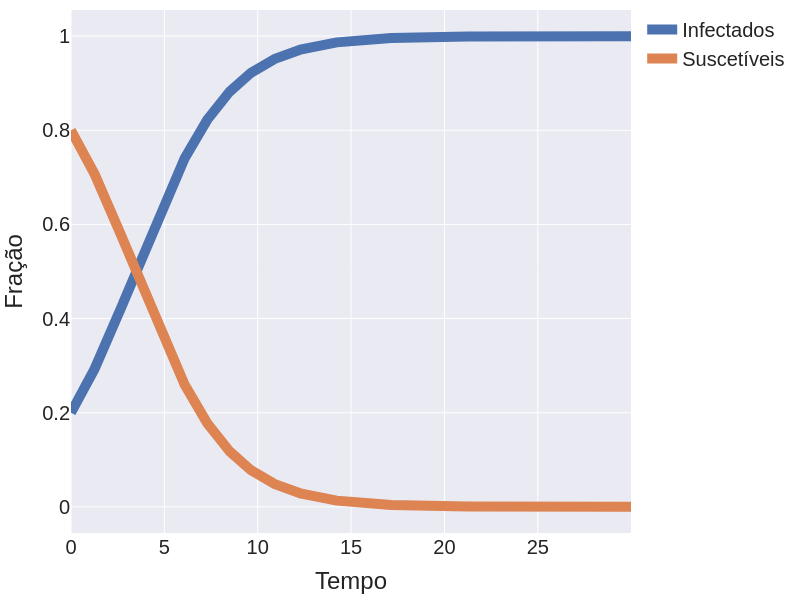
\includegraphics[scale=0.5]{figuras/SI.png}
  \captionsetup{font=small,position=below,skip=-1pt}
   \caption*{Gráfico que apresenta a evolução da infecção de um modelo SI com $I(0) = 0.2$ e $\overline{\beta} = 0.4$. Ele ilustra o crescimento de infectados ao longo do tempo em um modelo SI. Indica que, no início, há uma fração de infectados, e com o tempo, todos os indivíduos se tornarão infectados.\\Fonte: Autor.}
   \label{SI}
\end{figure}

Este modelo simplificado proporciona uma visão introdutória das dinâmicas de crescimento exponencial das infecções, ele se comporta bem 
para a modelagem de HIV~\cite{modelos} pois ou o indivíduo ao contrair a doença se torna imune ou porque após infectado jamais retorna para o compartimento de suscetível. Apesar disso ainda existem várias outras doenças que não são modeladas dessa maneira.

\subsection{Modelo SIS}

\begin{figure}[ht]
  \centering
  
  \captionsetup{font=normalsize,skip=0.8pt,singlelinecheck=on,labelsep=endash}
  \caption{Esquematização do Modelo Susceptível-Infectado-Susceptível de contágio.} 
  \begin{tikzpicture}

    \draw[->] (2,2.7) -- node[above] {$\overline{\beta}$} (3.9,2.7) ;
    \draw[->] (4.1,2.4) -- node[below] {$\overline{\gamma}$} (2.1,2.4) ;
    
    \draw[rounded corners,drop shadow, fill=ninfect,draw=border, ultra thick] (0,2) rectangle (2,3)node[pos=.5,text= white,font=\fontsize{20}{20}\selectfont]  {$S$};
    
    \draw[rounded corners,drop shadow, fill=infect,draw=border, ultra thick](4, 2) rectangle (6,3) node[pos=.5,text= white,font=\fontsize{20}
    {20}\selectfont]  {$I$};
  \end{tikzpicture}
  \label{img:SIS_}
\end{figure}

O modelo SIS, esquematizado na Figura \ref{img:SIS_},  é o modelo matemático 
que descreve a dinâmica de uma população dividida em dois compartimentos suscetíveis (S) e infectados (I) na qual é possível um indivíduo passar de infectado e voltar a ser suscetível, criando um ciclo contínuo de infecção e recuperação na população. São exemplos de doenças que podem ser modeladas a meningite, doenças venéreas e tuberculose~\cite{modelos}. O modelo segue com uma lógica idêntica ao SI adicionando um termo $\overline{\gamma}$ que representa a taxa de recuperação do indivíduo, obtendo o seguinte conjunto de equações:
\begin{align}
\frac{dS}{dt} &= -\overline{\beta} \cdot S \cdot I+ \overline{\gamma} \cdot I, \label{SIS-1} \\
\frac{dI}{dt} &= +\overline{\beta} \cdot S \cdot I- \overline{\gamma} \cdot I.\label{SIS-2} 
\end{align}
A partir desse conjunto de equações ainda é possível encontrar uma solução analítica,
obtendo as seguintes 
expressões 
para $S$ e $I$:
\begin{align}
I(t) &= \left(1 - \frac{\overline{\gamma}}{\overline{\beta}}\right)\frac{Ce^{(\overline{\beta} - \overline{\gamma})t}}{1 + Ce^{(\overline{\beta} - \overline{\gamma})t}}, \\
S(t) &= 1 - I(t).
\label{SIS_resolvido}
\end{align}
com 
$C = I(0)/(1 - I(0) - \overline{\gamma}/\overline{\beta})$. Assim a Equação \ref{SIS_resolvido} têm três tipos de comportamento dependendo de $\overline{\beta}$ e de $\overline{\gamma}$. Se $\overline{\beta} = \overline{\gamma}$ significa que a taxa de indivíduos que se tornam infectados é equivalente à taxa de recuperação que faz com que os infectados voltem a ser suscetíveis. Transforma as duas equações em $I = \frac{I(0)}{I(0)+ \overline{\beta} t}$ e $S(t) = \frac{\overline{\beta} t}{1 - S(0) + \overline{\beta} t}$ que mostra que a fração de infectados decai com $1/t$ e quando tempo tende a infinito o número de infectados tende para zero enquanto os suscetíveis converge para o tamanho da amostra. 
Se $\overline{\beta} > \overline{\gamma}$, significa que a taxa de infecção é maior que a de recuperação, e para $t \rightarrow \infty$ converge para um equilíbrio estável na qual $I(\infty) = 1 - \frac{\overline{\gamma}}{\overline{\beta}}$ e $S(\infty) = \frac{\overline{\gamma}}{\overline{\beta}}$, ou seja mesmo no infinto  ainda existirá a doença no modelo
(veja Fig. \ref{SIS}). 
Se $\overline{\beta} < \overline{\gamma}$, ou seja, a taxa de recuperação é maior que a taxa de infecção, e para $t \rightarrow \infty$ o número de infectados tende a 0 e o de suscetíveis tende a 1, ou seja, livre da doença 
(veja Fig. \ref{SIS_2}).

\begin{figure}[H]
  \centering
  \captionsetup{font=normalsize,skip=1pt,singlelinecheck=on,labelsep=endash}
  \caption{Modelo SIS}
  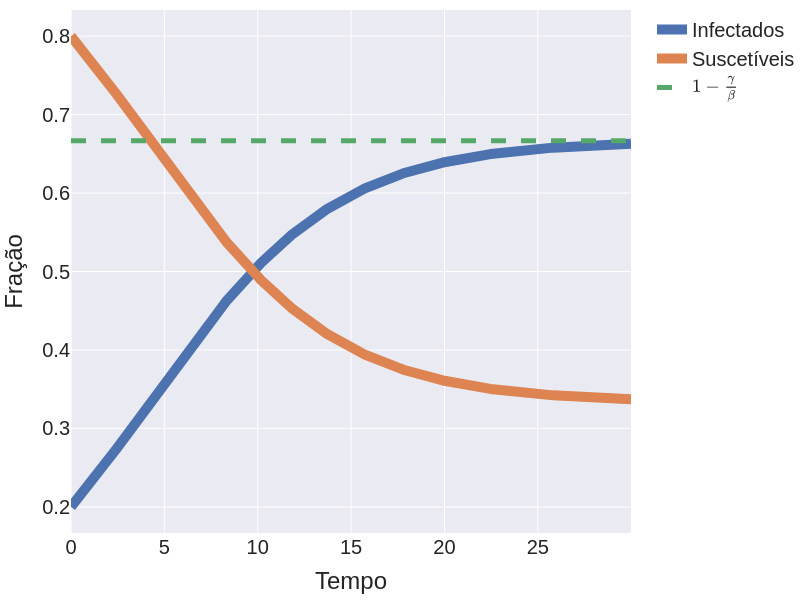
\includegraphics[scale=0.4]{figuras/SIS_1.png}
   \caption*{Gráfico que apresenta a evolução da infecção de um modelo 
   SIS com $I(0) = 0.2$, $\overline{\beta} = 0.3$ e $\overline{\gamma} = 0.1$. Nele existe convergência para equilíbrio estável no modelo SIS, com $\overline{\beta} > \overline{\gamma}$. Para $t \rightarrow \infty$, as frações de infectados e suscetíveis estabilizam em $1 - \frac{\overline{\gamma}}{\overline{\beta}}$ e $\frac{\overline{\gamma}}{\overline{\beta}}$ respectivamente, indicando persistência da doença em um horizonte infinito.\\Fonte: Autor.}
   \label{SIS}
\end{figure}


\begin{figure}[H]
  \centering
  \captionsetup{font=normalsize,skip=1pt,singlelinecheck=on,labelsep=endash}
  \caption{Modelo SIS}
  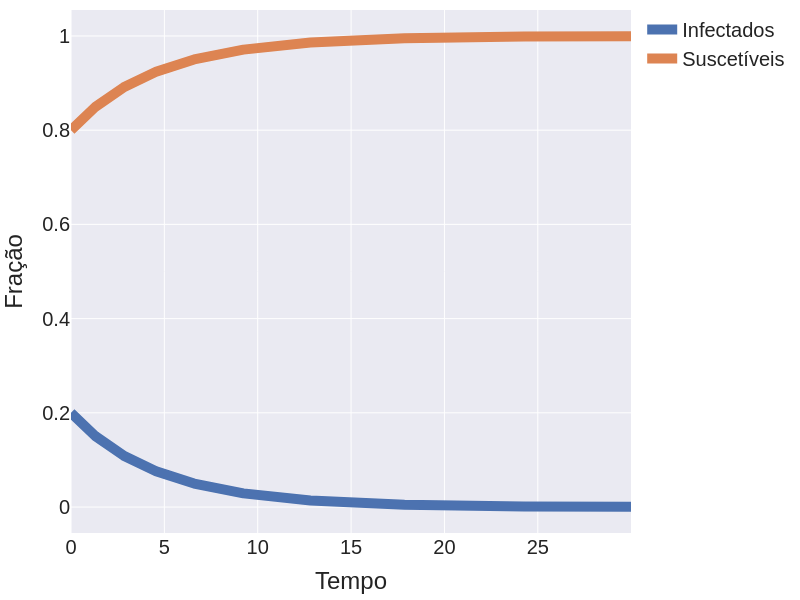
\includegraphics[scale=0.4]{figuras/SIS_2.png}
  \captionsetup{font=small,position=below,skip=-1pt}
   \caption*{Gráfico que apresenta a evolução da infecção de um modelo SIS com $I(0) = 0.2$, $\overline{\gamma} = 0.3$ e $\overline{\beta} = 0.1$. Caso $\overline{\beta} < \overline{\gamma}$, com a taxa de recuperação maior que a taxa de infecção, para $t \rightarrow \infty$, o número de infectados se aproxima de zero e o de suscetíveis se aproxima de um, indicando a erradicação da doença.\\Fonte: Autor.}
   \label{SIS_2}
\end{figure}

\subsection{Modelo SIR}


Por fim o último dos modelos básicos para o estudo de infecções é inspirado por doenças que após a infecção o indivíduo deixa de ser infectado, contudo, não pode ser infectado novamente, isso pode ter a interpretação de que o indivíduo ganhou imunidade ou morreu.
Esse
modelo é o SIR (suscetível, infectado e removido) na qual adiciona um novo compartimento R, conforme esquematização da Figura~\ref{img:SIR_}. Um exemplo de doença que pode ser modelada é a catapora no qual um indivíduo após infectado fica imune à enfermidade.

\begin{figure}[ht]
  \centering
  \captionsetup{font=normalsize,skip=0.8pt,singlelinecheck=on,labelsep=endash}
  \caption{Esquematização do Modelo Susceptível-Infectado-Removido de contágio.} 
  \begin{tikzpicture}

    \draw[->] (2,2.5) -- node[above] {$\overline{\beta}$} (3.9,2.5) ;
    \draw[->] (6.1,2.5) -- node[above] {$\overline{\omega}$} (7.9,2.5) ;
    
    \draw[rounded corners,drop shadow, fill=ninfect,draw=border, ultra thick] (0,2) rectangle (2,3)node[pos=.5,text= white,font=\fontsize{20}{20}\selectfont]  {$S$};
    
    \draw[rounded corners,drop shadow, fill=infect,draw=border, ultra thick](4, 2) rectangle (6,3) node[pos=.5,text= white,font=\fontsize{20}
    {20}\selectfont]  {$I$};
    \draw[rounded corners,drop shadow, fill=infect,draw=border, ultra thick](8, 2) rectangle (10,3) node[pos=.5,text= white,font=\fontsize{20}
    {20}\selectfont]  {$R$};
  \end{tikzpicture}
  \label{img:SIR_}
\end{figure}

O modelo SIR pode ser descrito pelas equações
\begin{align}
\frac{dS}{dt} &= -\overline{\beta} \cdot S \cdot I\\
\frac{dI}{dt} &= +\overline{\beta} \cdot S \cdot I- \overline{\omega} \cdot I\\
\frac{dR}{dt} &= +\overline{\omega} \cdot I\\
S +I+ R &= 1,
\label{SIR}
\end{align}
com $I(0) = I_0$, $R(0) = 0$ e $S(0) = S_0$ e $\overline{\omega}$ a taxa de remoção. Diferente dos modelos anteriores, esse não tem solução analítica para a equação diferencial acoplada precisando de uma solução usando métodos computacionais, contudo ainda é possível extrair análises a partir dessas equações. A partir da equação $\frac{dI}{dt}$ e igualando ela a zero existe um ponto crítico de máximo em $S = \frac{\overline{\omega}}{\overline{\beta}}$ que não aparecia nos modelos anteriores, enquanto $S > \frac{\overline{\omega}}{\overline{\beta}}$ o modelo apresenta numa fase endêmica, na qual o número de infectados cresce até chegar no ponto crítico, quando $S < \frac{\overline{\omega}}{\overline{\beta}}$ o número de infectados decresce até chegar no final da endemia. Esse valor crítico é chamado de número ou taxa de reprodutibilidade basal $R_0$ que representa o número médio de pessoas que são infectadas por um único indivíduo. 

\begin{figure}[H]
  \centering
  \captionsetup{font=normalsize,skip=1pt,singlelinecheck=on,labelsep=endash}
  \caption{Modelo SIR}
  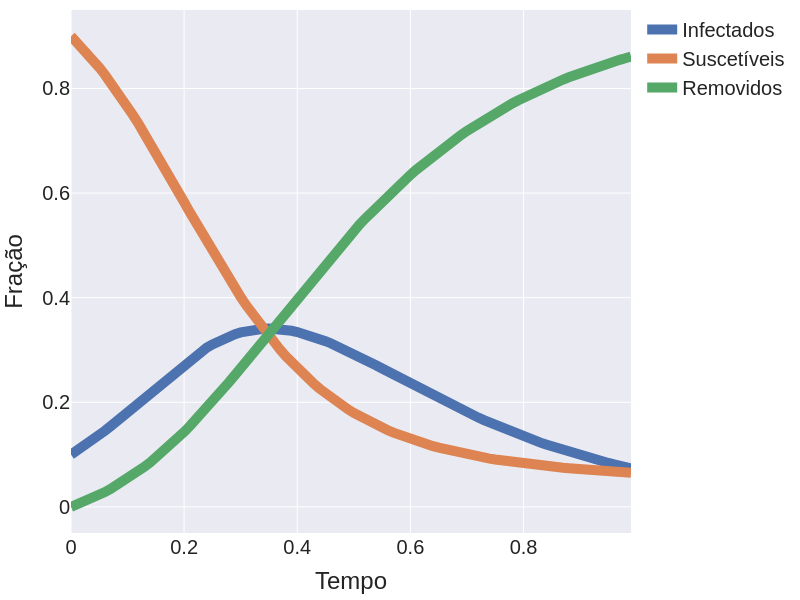
\includegraphics[scale=0.5]{figuras/SIR.png}
  \captionsetup{font=small,position=below,skip=-1pt}
   \caption*{Gráfico que apresenta a evolução da infecção de um modelo SIR com $I(0) = 0.2$,$S(0) = 0.8$, 
   $R(0) = 0$, $\overline{\omega} = 0.4$ e $\overline{\beta} = 1.2$. É mostrado existe um ponto de máximo de I(t), esse gráfico é bastante sensível aos parâmetros e seu comportamento pode mudar bastante com a alteração deles.  \\Fonte: Autor.}
   \label{img:SIR}
\end{figure}

\subsection{Modelos em Redes}

%PIF17042024 Acho que esta sub-seção precisa mais referências: a área de difusão de doenças em redes é muito ampla.
% Citar sobre outras modelagens em Redes

Toda a modelagem descrita anteriormente foi apresentada no contexto de equações diferenciais, porém ela tem as suas limitações como discutido anteriormente, contudo elucidam bem sobre como é feita esse tipo de modelagem. No contexto de redes complexas existem duas formas de construir a 
modelagem~\cite{networks}: 
de tempo contínuo ou de tempo discreto. 
Por exemplo, num modelo SI 
cada nó vai receber um rótulo descrevendo em qual compartimento ele está. No caso de tempo discreto um nó
$\nu$ 
no compartimento S tem uma
probabilidade $p = (1 - \beta)^{k^I_\nu}$ de não ser contaminado, na qual $\beta$ é diferente do que aparece nas equações diferenciais, enquanto no modelo de redes ele é uma probabilidade associada ao indivíduo, na modelagem por equações diferenciais é algo médio para todo o sistema, isso se aplica também ao $\gamma$ e $\omega$ e $k_\nu^I$ é o número de vizinhos de $\nu$ que estão no estágio $I$. Portanto, a probabilidade de ser contaminado por pelo menos um nó é de
\begin{equation}
    p_\nu = 1 - (1 - \beta)^{k^I_\nu}.
\end{equation}
Uma vez calculada a probabilidade de contágio, pode-se decidir se o vértice passará ao estado I, em cujo caso muda-se o próximo estado do vértice para I. Ou seja, depois de uma interação no modelo na qual passa uma unidade de tempo (depende da unidade de $\beta$) os nós suscetíveis 
têm 
probabilidade $p_i$ de serem contaminados, por isso é chamado de tempo discreto. No caso do modelo SIR ou SIS, existe uma probabilidade $\gamma$ ou $\omega$ dele sair do estado infectado. Contudo, essa probabilidade não depende dos seus vizinhos, então cada nó que esteja infectado tem uma probabilidade $\gamma$ ou $\omega$ de depois de uma unidade de tempo de mudar de estágio. O Algoritmo \ref{algoritmo:discreto} mostra um pseudo-código de como funciona para o caso discreto o modelo SIS.

\begin{algorithm}[htbp]
   \caption{Algoritmo caso discreto do modelo SIS}
   \label{algoritmo:discreto}
   \SetKwInOut{Input}{Input}
\Input{$G(\mathpzc{N} ,\mathpzc{L})$: rede.}
\Input{$random()$: função que retorna um número ao acaso em $(0,1)$.}

   \For{$\nu_i \in \mathpzc{N}$}{
      $\mathrm{estado}[i] \gets$ Inicialização de estados; \tcp{S ou I}
   }
   $t \gets 0$\\
   \While{$t \leq tempo$}{
      \For{$\nu_i \in \mathpzc{N}$}{ 
         \eIf{$\mathrm{estado}[i] = S$}{
            $\mathrm{num\_inf}\gets 0$\\
            \For{$\nu_j \in \eta(\nu_i)$}{
                \If{$\mathrm{estado}[j] = I$}{
                    $\mathrm{num\_inf}\gets \mathrm{num\_inf}+1$\\
                }
            }
            $p \gets 1 - (1 - \beta)^{\mathrm{num\_inf}}$\\
            
            \If{$random() < p$}{
               $\mathrm{estado}[i] \gets I$\\
            }
         }{
            \If{$random() < \gamma$}{
               $\mathrm{estado}[i] \gets S$\\
            }
         }
      }
      $t \gets t + 1$\\
   }
\end{algorithm}

Para tempo contínuo no modelo SI,tradicionalmente , cada nó tem um tempo 
$T_{\nu}^{s\rightarrow i} \sim \mathrm{Exp}(k_\nu^I\beta)$ (distribuição exponencial com parâmetro $k_\nu^I\beta$) para ser contaminado,
com $k_\nu^I = |I\cap \eta(\nu)|$ (contudo há estudos com tempos não exponenciais \cite{feng2007epidemiological}). Portanto, o tempo $\Delta t$ para a próxima atualização na rede segue uma distribuição exponencial com parâmetro a soma dos parâmetros de cada variável
$\Delta t \sim \mathrm{Exp}(\sum_{\nu \in S}k_\nu^I\beta)$,
pois o mínimo entre várias variáveis exponenciais independentes segue uma distribuição exponencial com a soma dos parâmetros.

A escolha do nó a ser atualizado é feita a partir do cálculo de 
$M = \sum_{\nu \in S}k_\nu\beta$.
Seja $S = \{\mu_1,\mu_2,\cdots,\mu_{|S|}\}$ uma ordem do conjunto de nós suscetíveis. Assim é gerado um valor $r$ aleatório entre 0 e 1, o nó $\mu_j$ a ser atualizado é primeiro vértice tal que $\sum_{i=1}^{j}k_{\mu_i}^I\beta \geq r\cdot M$. Para modelos como SIS e SIR segue a mesma ideia, sem considerar os vizinhos, o tempo para mudar de estágio é $T_{\nu}^{i\rightarrow s} \sim \mathrm{Exp}(\gamma)$ ou $T_{\nu}^{i\rightarrow r} \sim \mathrm{Exp}(\omega)$, agora $M$ é calculado com a soma de $\sum_{\nu \in S}k_\nu^I\beta+ \sum_{\nu \in I}\gamma$ ou de $\sum_{\nu \in S}k_\nu^I \beta+ \sum_{\nu \in I}\omega$ e assim o tempo que passa é $\Delta t \propto \mathrm{Exp}(M)$ e o nó escolhido é tal que a soma de todas as taxas até ele seja maior que $r\cdot M$~\cite{Gillespie1976}. O Algoritmo \ref{algoritmo:continuo} mostra um pseudo-código de como funciona para o caso contínuo o modelo SIS.


\begin{algorithm}[htbp]
   \caption{Algoritmo caso contínuo do modelo SIS}
   \label{algoritmo:continuo}
   \SetKwInOut{Input}{Input}
\Input{$G(\mathpzc{N} ,\mathpzc{L})$: rede.}
\Input{$random()$: função que retorna um número ao acaso em $(0,1)$.}
\Input{$exp(\lambda)$: função que retorna um número aleatório com distribuição exponencial de parâmetro $\lambda$.}
   \For{$\nu \in\mathpzc{N}$}{
      \tcp{Inicialização de estados}
      $S \gets S\cup \{\nu\}$ ou  $I \gets I\cup \{\nu\}$
   }
   $t \gets 0$\\
   \While{$t \leq tempo$}{
      $M \gets 0$\\
      \tcp{Os nós são visitados numa ordem fixa}
      \For{$\nu_i \in \mathpzc{N}$}{
         \eIf{$\nu_i \in S$}{
            $k_{\nu_i}^I \gets |I\cap \eta(\nu_i)|$\\
            $\mathrm{rate}[i] \gets k_\nu^I \cdot \beta$\\
         }{
            $\mathrm{rate}[i] \gets \gamma$\\
         }
         $M \gets M + \mathrm{rate}[i]$\\
      }
      $t \gets t + exp(M)$\\
      $\Delta \gets random() \cdot M$\\
      $m \gets 0$\\
      $i \gets 0$\\
      \While{$m \leq \Delta$}{
         $i \gets i + 1$\\
         $m \gets m + \mathrm{rate}[i]$\\
      }
      \eIf{$\nu_i \in S$}{
         $I \gets I\cup\{\nu_i\}$\\
         $S \gets S\setminus\{\nu_i\}$\\
      }{
         $S \gets S\cup\{\nu_i\}$\\
         $I \gets I\setminus\{\nu_i\}$\\
      }
   }
\end{algorithm}
